\documentclass[11pt,a4paper,titlepage]{article}
\usepackage[T1]{fontenc}
\usepackage[czech]{babel}        % česká dělení slov, názvy (Obrázek, Tabulka, Obsah)
\usepackage{lmodern}             % písmo s českými znaky
\usepackage[margin=2.5cm]{geometry}
\usepackage{amsmath}             % rovnice
\usepackage{amssymb}             % matematické symboly (např. \mathbb{R})
\usepackage{graphicx}            % obrázky
\usepackage{booktabs}            % tabulky
\usepackage{tikz}                % schémata
\usetikzlibrary{arrows.meta, fit}
\usepackage{csquotes}            % uvozovky (vyžaduje biblatex)
\usepackage[style=numeric]{biblatex} % citace [1], [2], ...
\usepackage[hidelinks]{hyperref} % odkazy v PDF (bez rámečků)

\graphicspath{{images/}}         % obrázky se hledají ve složce images
\addbibresource{references.bib}  % soubor se zdroji

\title{Úvod do deep learningu -- Predikce úspěchu her na Steamu}
\author{Marek Szczepanik}
\date{\today}

\begin{document}

\maketitle

\tableofcontents
\newpage

\section{Formulace úlohy}

Cílem projektu je odhadnout popularitu hry na Steamu z informací dostupných už v době jejího
vydání: z metadat a z obrázků, kterými se hra prezentuje na své stránce (header a tři screenshoty).
Hlavní otázkou je, zda obrázky nesou informaci o popularitě navíc oproti samotným metadatům.

Steam nezveřejňuje počty prodaných kopií, proto jsem jako míru popularity zvolil celkový počet
recenzí. Jeho rozdělení je extrémně zešikmené (většina her má jednotky recenzí, několik her
miliony), a proto predikuji jeho logaritmus:
\begin{equation}
    y_i = \log\left(1 + r_i^{+} + r_i^{-}\right),
\end{equation}
kde $r_i^{+}$ a $r_i^{-}$ jsou počty pozitivních a negativních recenzí hry $i$. Chyba na této
škále vyjadřuje relativní rozdíl, takže malá i velká hra mají při trénování srovnatelnou váhu.

Úloha je regrese. Model s parametry $\theta$ předpovídá
$\hat{y}_i = f_\theta(\mathbf{m}_i, \mathbf{I}_i) \in \mathbb{R}$, kde $\mathbf{m}_i \in \mathbb{R}^{77}$
jsou metadata a $\mathbf{I}_i$ čtyři obrázky o rozměru $3 \times 128 \times 128$. Výstupem je
jedno reálné číslo bez výstupní aktivace. Parametry učím minimalizací průměrné ztráty
na trénovací množině o $n$ hrách:
\begin{equation}
    \min_\theta \; L(\theta) = \frac{1}{n} \sum_{i=1}^{n} \ell_\delta\left(\hat{y}_i, y_i\right), \qquad
    \ell_\delta(\hat{y}, y) =
    \begin{cases}
        \frac{1}{2}(\hat{y} - y)^2 & \text{pro } |\hat{y} - y| \le \delta, \\
        \delta \left(|\hat{y} - y| - \frac{1}{2}\delta\right) & \text{jinak,}
    \end{cases}
\end{equation}
kde $\ell_\delta$ je Huberova ztráta~\cite{huber1964} s $\delta = 1$. Zvolil jsem ji, protože se
u malých chyb chová jako kvadratická ztráta, ale velké chyby penalizuje jen lineárně. Hry
s nečekaně vysokou popularitou, kterou ze vstupů nelze předpovědět, tak neovládnou trénování.

Modely vyhodnocuji pomocí MAE a RMSE na logaritmické škále. MAE je hlavní metrikou, protože
se dobře interpretuje: chyba 1 znamená odhad počtu recenzí, který se od skutečnosti liší
přibližně $e \approx 2{,}7$krát. RMSE silněji penalizuje velké chyby, a ukazuje tak, jak si model
vede u extrémních případů. Model i nejlepší epochu vybírám jen podle validační množiny.
\section{Data}

\subsection*{Zdroj}

Projekt vychází z datasetu Steam Games Dataset~\cite{fronkon_dataset}, který obsahuje metadata
her získaná přes API Steamu. Použit je soubor \texttt{games.json} v pevné revizi, aby byla data
reprodukovatelná. Soubor obsahuje 148\,909 záznamů a 42 sloupců. Kromě metadat obsahuje
i odkazy na obrázky hry: header a seznam screenshotů.

\subsection*{Čištění}

Hry s nulovým počtem recenzí nelze použít, protože nulu nelze odlišit od chybějících dat:
3\,467 her má nulový počet recenzí, ačkoli má nenulový počet doporučení
(\texttt{recommendations}). Podíl takových chybějících hodnot navíc roste u novějších her.
Medián poměru počtu recenzí a počtu doporučení v letech 2011--2023 pozvolna klesá z 1,43 na 1,06,
od roku 2024 ale výrazně klesá (0,99 v roce 2024, 0,81 v roce 2025). Počty recenzí novějších her
jsou tedy podhodnocené, a proto se data omezují na hry vydané do roku 2023. Postup čištění
a počty her po jednotlivých krocích shrnuje tabulka~\ref{tab:cisteni}.

\begin{table}[h]
    \centering
    \begin{tabular}{lr}
        \toprule
        Krok & Počet her \\
        \midrule
        Původní data & 148\,909 \\
        Vydáno do roku 2023 & 77\,575 \\
        Alespoň 1 recenze & 64\,675 \\
        Alespoň 3 screenshoty a header & 64\,554 \\
        Bez softwaru (pouze softwarové žánry) & 63\,889 \\
        Bez duplicit (stejný název a vývojář) & 63\,804 \\
        \bottomrule
    \end{tabular}
    \caption{Počet her po jednotlivých krocích čištění.}
    \label{tab:cisteni}
\end{table}

U stejné hry vedené pod více identifikátory zůstává záznam s nejvíce recenzemi. Seznam
podporovaných jazyků obsahoval chybně zapsané položky (zbytky HTML a BBCode, více jazyků
v jedné položce), názvy jazyků se z nich proto extrahují regulárním výrazem.

\subsection*{Rozdělení dat}

Data jsou rozdělena časově podle roku vydání (tabulka~\ref{tab:rozdeleni}). Model se tak
vyhodnocuje na hrách vydaných později než trénovací data, což odpovídá praktickému použití
(predikce pro nově vydávané hry). Jednotkou rozdělení je hra, každá hra je tedy právě v jedné
množině.

\begin{table}[h]
    \centering
    \begin{tabular}{lcrr}
        \toprule
        Množina & Roky vydání & Počet her & Podíl \\
        \midrule
        Trénovací & do 2021 & 45\,565 & 71,4\,\% \\
        Validační & 2022 & 8\,611 & 13,5\,\% \\
        Testovací & 2023 & 9\,628 & 15,1\,\% \\
        \bottomrule
    \end{tabular}
    \caption{Časové rozdělení dat.}
    \label{tab:rozdeleni}
\end{table}

\subsection*{Vstupy modelu}

Metadata jsou zakódována do 77 vstupů:
\begin{itemize}
    \item standardizovaný rok vydání, $\log(1 + \text{cena})$ a $\log(1 + \text{počet jazyků})$,
    \item binární příznaky: hra zdarma, podpora Windows, macOS a Linuxu,
    \item multi-hot 22 žánrů s alespoň 50 hrami v trénovací množině,
    \item multi-hot 19 kategorií popisujících design hry (např. Single-player, Co-op, VR),
    \item multi-hot 29 jazyků podporovaných alespoň 1\,\% her v trénovací množině.
\end{itemize}

Obrazovým vstupem je header a první tři screenshoty každé hry. Obrázky jsou zmenšeny,
oříznuty na střed na čtverec $128 \times 128$ pixelů a jejich hodnoty škálovány do intervalu
$[0, 1]$.

\subsection*{Prevence úniku informací}

Vstupy obsahují pouze informace známé v době vydání hry. Vyřazeny jsou počty doporučení,
vlastníků, souběžných hráčů, herní doba, uživatelské tagy a počet DLC, které vznikají až po
vydání a souvisí s popularitou. Z kategorií jsou použity jen ty, které popisují design hry.
Kategorie přidávané až později (např. Steam Trading Cards nebo Remote Play) by popularitu
prozrazovaly. Ze stejného důvodu je vyřazen žánr Early Access, který odpovídá stavu hry
v době stažení dat. Parametry kódování (seznamy žánrů a jazyků, průměry a směrodatné
odchylky) se počítají pouze z trénovací množiny.

\subsection*{Omezení dat}

\begin{itemize}
    \item Počet recenzí je jen nepřímou mírou popularity. Starší hry měly na sběr recenzí
    více času, průměrné $y$ proto s rokem vydání klesá (v trénovací množině z 7,35 v roce 2013
    na 3,39 v roce 2021).
    \item Vyřazením her bez recenzí se model učí jen na hrách s alespoň jednou recenzí
    a pro hry bez recenzí jeho predikce neplatí.
    \item Rok vydání validačních a testovacích her leží mimo rozsah trénovací množiny
    (po standardizaci průměrně 1,51 a 1,90 směrodatné odchylky), model tedy musí extrapolovat.
    \item Obrázky odpovídají stavu stránky hry v době stažení. Vývojáři je mohli po vydání
    změnit, takže nemusí přesně odpovídat prezentaci v době vydání.
\end{itemize}
\section{Modely a trénování}

\subsection*{Baseline}

Jako referenční modely slouží čtyři přístupy pracující jen s metadaty. Nejjednodušší baseline
předpovídá pro každou hru průměr $y$ z trénovací množiny. Dále je použita lineární regrese
a gradient boosting (\texttt{HistGradientBoostingRegressor} s výchozím nastavením) z knihovny
scikit-learn~\cite{pedregosa2011sklearn}. Poslední baseline je neuronová síť MLP se skrytou
vrstvou o 128 neuronech a aktivací ReLU (10\,113 parametrů). Ta je zároveň referencí pro otázku,
zda obrázky přinášejí informaci navíc.

\subsection*{Hybridní architektura}

Modely A a B sdílejí stejnou hybridní architekturu (obrázek~\ref{fig:architektura}) a liší se
pouze encoderem obrázků. Encoder $e_\psi$ převede každý ze čtyř obrázků na vektor délky $d$.
Vektory se zprůměrují, spojí s metadaty a MLP hlava $g_\phi$ z nich spočítá predikci:
\begin{equation}
    \hat{y}_i = g_\phi\left(\left[\frac{1}{4} \sum_{k=1}^{4} e_\psi(I_{i,k}) \,;\, \mathbf{m}_i\right]\right),
\end{equation}
kde $[\,\cdot\,;\,\cdot\,]$ značí spojení vektorů. Jeden encoder zpracovává všechny obrázky,
takže se počet jeho parametrů s počtem obrázků nezvyšuje. Průměrování navíc nezávisí na pořadí
obrázků. Hlava $g_\phi$ má stejnou strukturu jako baseline MLP: lineární vrstvu s $h$ výstupy,
ReLU a lineární výstupní vrstvu s jedním neuronem. Šířka $h$ je hyperparametr (kapitola~4),
ve finálních konfiguracích obou modelů je $h = 64$.

\begin{figure}[h]
    \centering
    \begin{tikzpicture}[
        box/.style={draw, rounded corners, align=center, minimum height=8mm, inner sep=3pt, font=\small},
        arr/.style={-Stealth}
    ]
        % čtyři obrázky hry a sdílený encoder
        \foreach \i/\name in {1/header, 2/screenshot 1, 3/screenshot 2, 4/screenshot 3} {
            \node[box, minimum width=2.3cm] (img\i) at (0, {-(\i-1)*1.1}) {\name};
            \node[box, fill=blue!10, minimum width=1.8cm] (enc\i) at (2.9, {-(\i-1)*1.1}) {$e_\psi$};
            \draw[arr] (img\i) -- (enc\i);
        }
        \node[draw, dashed, rounded corners, inner sep=5pt, fit=(enc1)(enc4),
              label={[font=\small]above:encoder (sdílené váhy)}] {};

        % průměr vektorů obrázků a spojení s metadaty
        \node[box] (mean) at (5.6, -1.65) {průměr\\$\mathbb{R}^{d}$};
        \foreach \i in {1,...,4} \draw[arr] (enc\i.east) -- (mean.west);
        \node[box] (meta) at (5.6, -4.0) {metadata\\$\mathbb{R}^{77}$};
        \node[box] (cat) at (8.0, -2.8) {spojení\\$\mathbb{R}^{d+77}$};
        \draw[arr] (mean) -- (cat);
        \draw[arr] (meta) -- (cat);

        % MLP hlava a výstup
        \node[box, fill=orange!15] (head) at (10.9, -2.8) {hlava $g_\phi$\\Linear($h$), ReLU\\Linear(1)};
        \draw[arr] (cat) -- (head);
        \node (out) at (13.0, -2.8) {$\hat{y}$};
        \draw[arr] (head) -- (out);
    \end{tikzpicture}
    \caption{Hybridní architektura modelů A a B. Sdílený encoder převede každý obrázek na vektor
    délky $d$ ($d = 64$ pro model A, $d = 768$ pro model B), vektory se zprůměrují a spojí s metadaty.}
    \label{fig:architektura}
\end{figure}

\subsection*{Model A: vlastní CNN}

Encoder modelu A je konvoluční síť trénovaná od náhodné inicializace. Skládá se ze tří bloků,
každý obsahuje dvě konvoluce $3 \times 3$ s aktivací ReLU a max pooling $2 \times 2$, který
zmenšuje prostorové rozlišení na polovinu. Počet kanálů se v blocích zdvojnásobuje
(16, 32, 64), rozlišení klesá ze $128 \times 128$ na $16 \times 16$. První bloky zachycují
jednoduché vzory (hrany, barvy, textury), další bloky z nich skládají složitější struktury.
Global average pooling zprůměruje každou ze 64 map příznaků na jedno číslo. Výsledný vektor
tak popisuje, \emph{zda} se vzor v obrázku vyskytuje, ale ne \emph{kde}. Následují dvě plně
propojené vrstvy (64 $\rightarrow$ 128 $\rightarrow$ 64) s aktivací ReLU, takže $d = 64$.

Global average pooling nahradil v původní verzi sítě natažení map příznaků do plně propojené
vrstvy s přibližně 4,2 milionu parametrů, se kterou se síť rychle přeučovala.

\subsection*{Model B: předtrénovaný encoder}

Model B používá jako encoder síť ConvNeXt-Tiny~\cite{liu2022convnext} předtrénovanou
na datasetu ImageNet~\cite{deng2009imagenet} z knihovny torchvision. Klasifikační vrstva
pro 1000 tříd je odstraněna, výstupem je vektor délky $d = 768$. Váhy encoderu jsou zmrazené,
trénuje se pouze hlava $g_\phi$ (linear probing s MLP hlavou). Obrázky se normalizují
statistikami ImageNetu. Encoder zůstává i během trénování v režimu inference, aby se nepoužíval
stochastic depth, který náhodně vynechává bloky sítě. Síť byla předtrénována na obrázcích
$224 \times 224$, zde dostává obrázky $128 \times 128$.

\begin{table}[h]
    \centering
    \begin{tabular}{lrrr}
        \toprule
        Model & Encoder & Hlava & Trénované \\
        \midrule
        MLP (metadata) & -- & 10\,113 & 10\,113 \\
        Model A & 88\,656 & 9\,153 & 97\,809 \\
        Model B & 27\,820\,128 & 54\,209 & 54\,209 \\
        \bottomrule
    \end{tabular}
    \caption{Počty parametrů modelů ve finálních konfiguracích (hlava modelů A a B s $h = 64$).}
    \label{tab:parametry}
\end{table}

\subsection*{Trénování}

Všechny neuronové sítě jsou implementovány v PyTorch~\cite{paszke2019pytorch} a trénovány
stejným postupem. Minimalizuje se Huberova ztráta (kapitola~1) optimizerem
AdamW~\cite{loshchilov2019adamw}, který aktualizuje parametry podle
\begin{equation}
    \theta_t = \theta_{t-1} - \eta \left( \frac{\hat{m}_t}{\sqrt{\hat{v}_t} + \epsilon} + \lambda \theta_{t-1} \right),
\end{equation}
kde $\hat{m}_t$ a $\hat{v}_t$ jsou korigované klouzavé průměry gradientu a jeho druhé mocniny,
$\eta$ je learning rate a $\lambda$ weight decay. Na rozdíl od L2 regularizace v původním
Adamu se weight decay neškáluje adaptivním krokem. MLP nad metadaty používá $\eta = 10^{-3}$,
$\lambda = 10^{-4}$ a velikost dávky 256. Hyperparametry modelů A a B jsou vybrány random
searchem (kapitola~4).

Po každé epoše se spočítá MAE na validační množině a ukládá se model z nejlepší epochy.
Trénování trvá nejvýše 15 epoch a končí dříve (early stopping), pokud se validační MAE
nezlepší 3 epochy po sobě. Dopředný průchod probíhá ve smíšené přesnosti (bfloat16), ztráta
se počítá ve float32. Formát bfloat16 má stejný rozsah exponentu jako float32, takže není
potřeba škálovat gradienty. Každý model je natrénován se třemi seedy
(123, 420, 666), které určují inicializaci vah i pořadí trénovacích dat.
\section{Experimenty}

\subsection*{Hledání hyperparametrů}

Hyperparametry jsou hledány metodou random search~\cite{bergstra2012random}. Oproti mřížkovému
hledání vyzkouší při stejném počtu běhů více různých hodnot každého hyperparametru, což je
výhodné, pokud výsledek ovlivňuje jen několik z nich. Hledání probíhá zvlášť pro model A a model B,
protože se optimální hodnoty (zejména learning rate) mezi encoderem trénovaným od nuly a malou
hlavou nad zmrazeným encoderem mohou výrazně lišit.

Prohledávaný prostor:
\begin{itemize}
    \item learning rate $\eta$: log-uniformně z intervalu $[10^{-4}, 3 \cdot 10^{-3}]$,
    \item weight decay $\lambda$: log-uniformně z intervalu $[10^{-5}, 10^{-2}]$,
    \item velikost dávky: $\{32, 64, 128\}$,
    \item šířka skryté vrstvy hlavy: $\{64, 128, 256\}$.
\end{itemize}
Learning rate a weight decay se vzorkují na logaritmické škále, protože jejich vliv závisí
na řádu hodnoty, ne na absolutním rozdílu. Každá konfigurace je natrénována s jedním seedem
a vyhodnocena podle MAE na validační množině. Pro každý model je vyzkoušeno 8 konfigurací.
Konfigurace se vzorkují se stejným seedem, takže oba modely dostávají stejné kombinace
hyperparametrů. Nejlepší konfigurace každého modelu je poté natrénována znovu se třemi seedy.

\begin{table}[h]
    \centering
    \begin{tabular}{crrrrrr}
        \toprule
        & $\eta$ & $\lambda$ & Dávka & $h$ & MAE A & MAE B \\
        \midrule
        1 & $1{,}02 \cdot 10^{-3}$ & $1{,}45 \cdot 10^{-5}$ & 128 & 64 & \textbf{1,1561} & 1,1407 \\
        2 & $1{,}87 \cdot 10^{-4}$ & $3{,}37 \cdot 10^{-5}$ & 64 & 256 & 1,1714 & 1,1425 \\
        3 & $2{,}31 \cdot 10^{-3}$ & $6{,}76 \cdot 10^{-5}$ & 128 & 256 & 1,1805 & 1,1538 \\
        4 & $2{,}06 \cdot 10^{-3}$ & $3{,}46 \cdot 10^{-4}$ & 32 & 64 & 1,1607 & 1,1450 \\
        5 & $1{,}65 \cdot 10^{-3}$ & $4{,}38 \cdot 10^{-5}$ & 64 & 256 & 1,1742 & 1,1474 \\
        6 & $8{,}52 \cdot 10^{-4}$ & $6{,}06 \cdot 10^{-3}$ & 128 & 64 & 1,1587 & \textbf{1,1393} \\
        7 & $1{,}51 \cdot 10^{-3}$ & $3{,}59 \cdot 10^{-4}$ & 128 & 64 & 1,1614 & 1,1443 \\
        8 & $1{,}76 \cdot 10^{-4}$ & $3{,}11 \cdot 10^{-4}$ & 32 & 128 & 1,1606 & 1,1521 \\
        \bottomrule
    \end{tabular}
    \caption{Random search: validační MAE osmi konfigurací (seed 123). Tučně nejlepší
    konfigurace každého modelu.}
    \label{tab:search}
\end{table}

Výsledky searche jsou v tabulce~\ref{tab:search}. Nejlepší je pro model A konfigurace~1 a pro
model B konfigurace~6, obě s velikostí dávky 128 a šířkou hlavy $h = 64$. Rozdíly mezi
konfiguracemi jsou malé: validační MAE se pohybuje mezi 1,156 a 1,181 u modelu A a mezi 1,139
a 1,154 u modelu B. U modelu A dosáhly nejvyšší chyby všechny tři konfigurace se šířkou hlavy 256.

\subsection*{Experiment 1: přínos jednotlivých modalit}

\textbf{Hypotéza:} Obrázky nesou informaci o popularitě, která v metadatech není. Model
kombinující obrázky s metadaty proto dosáhne nižší chyby než model nad samotnými metadaty.
Samotné obrázky budou méně informativní než metadata.

\textbf{Postup:} Porovnávají se tři varianty modelu B: pouze metadata, pouze obrázky a obě
modality. Varianta pouze s metadaty je samotná hlava $g_\phi$ bez encoderu, varianta pouze
s obrázky používá encoder ConvNeXt-Tiny a do hlavy vstupuje jen vektor obrázků. Všechny varianty
sdílejí stejné rozdělení dat, trénovací postup a hyperparametry nejlepší konfigurace modelu B. Každá varianta je natrénována se třemi seedy a vyhodnocena
pomocí MAE a RMSE na validační množině.

\subsection*{Experiment 2: encoder CLIP}

\textbf{Hypotéza:} Model CLIP~\cite{radford2021clip} je předtrénován kontrastivně na dvojicích
obrázků a textů z internetu, ne na klasifikaci do tříd ImageNetu. Jeho příznaky proto lépe
popisují vlastnosti propagačních obrázků her, jako je styl, žánr nebo kvalita zpracování.
Model B s encoderem CLIP dosáhne nižší chyby než s encoderem ConvNeXt-Tiny.

\textbf{Postup:} V modelu B je encoder ConvNeXt-Tiny nahrazen obrazovou částí modelu CLIP
ViT-B/32 s vahami od OpenAI z knihovny OpenCLIP~\cite{ilharco2021openclip}. Encoder je také
zmrazený a jeho výstupem je vektor délky $d = 512$. Obrázky $128 \times 128$ se zvětší
na $224 \times 224$, na kterých byl CLIP předtrénován, a normalizují se jeho průměrem
a směrodatnou odchylkou. Hlava, trénovací postup a hyperparametry nejlepší konfigurace modelu B
se nemění. Hyperparametry byly vybrány pro encoder ConvNeXt, což může CLIP mírně znevýhodnit.
Model je natrénován se třemi seedy a vyhodnocen pomocí MAE a RMSE na validační množině.

\section{Výsledky a diskuse}

\subsection*{Srovnání modelů}

\begin{table}[h]
    \centering
    \begin{tabular}{lcccc}
        \toprule
        Model & Val MAE & Val RMSE & Test MAE & Test RMSE \\
        \midrule
        Průměr & 1,783 & 2,130 & 1,869 & 2,208 \\
        Lineární regrese & 1,243 & 1,647 & 1,272 & 1,695 \\
        Gradient boosting & $1{,}189 \pm 0{,}002$ & $1{,}538 \pm 0{,}001$ & $1{,}284 \pm 0{,}001$ & $1{,}630 \pm 0{,}001$ \\
        MLP (metadata) & $1{,}179 \pm 0{,}001$ & $1{,}571 \pm 0{,}002$ & $1{,}230 \pm 0{,}005$ & $1{,}606 \pm 0{,}003$ \\
        Model A & $1{,}155 \pm 0{,}004$ & $1{,}532 \pm 0{,}009$ & $1{,}200 \pm 0{,}012$ & $1{,}575 \pm 0{,}010$ \\
        Model B & $1{,}144 \pm 0{,}006$ & $1{,}539 \pm 0{,}008$ & $1{,}183 \pm 0{,}007$ & $1{,}587 \pm 0{,}006$ \\
        Model B (CLIP) & $\mathbf{1{,}065} \pm 0{,}004$ & $\mathbf{1{,}436} \pm 0{,}005$ & $\mathbf{1{,}108} \pm 0{,}003$ & $\mathbf{1{,}481} \pm 0{,}006$ \\
        \bottomrule
    \end{tabular}
    \caption{Výsledky na validační (2022) a testovací (2023) množině: průměr $\pm$ směrodatná
    odchylka přes tři seedy. Průměr a lineární regrese jsou deterministické. Model B (CLIP)
    je varianta z experimentu~2.}
    \label{tab:vysledky}
\end{table}

Oba modely s obrázky dosahují na validační i testovací množině nižší MAE než všechny baseline
nad metadaty a pořadí podle MAE se mezi množinami nemění: model B, model A, MLP nad metadaty
(tabulka~\ref{tab:vysledky}). Na testovací množině má model B o 0,047 nižší MAE než MLP nad
metadaty, na validační o 0,035 (přibližně 5 a 4\,\% v odhadu počtu recenzí). Rozdíl mezi modely B a A (0,011 na validační a 0,017
na testovací množině) odpovídá přibližně jedno- až dvojnásobku směrodatné odchylky mezi seedy.
Při třech bězích jde o orientační výsledek, ne o prokázaný rozdíl.
Směrodatná odchylka je výběrová ($n - 1$) přes tři běhy, které se liší inicializací vah
a pořadím trénovacích dat, a vyjadřuje jen variabilitu mezi seedy. V RMSE je z modelů A a B
na obou množinách lepší model A. Varianta s encoderem CLIP z experimentu~2 si výhodu udržela
i na testovací množině (MAE o 0,075 nižší než model B) a je nejlepší ve všech metrikách.

Všechny modely mají na testovací množině vyšší chybu než na validační. Testovací hry leží rokem
vydání dál od trénovacích dat (kapitola~2). Nejvíce se zhoršil gradient boosting (MAE z 1,189
na 1,284), který je na testovací množině horší i než lineární regrese. Pravděpodobnou příčinou je,
že rozhodovací stromy nedokážou extrapolovat rok vydání mimo rozsah trénovací množiny, zatímco
lineární model ano. Neuronové sítě se zhoršily o 0,039 (model B) až 0,051 (MLP nad metadaty).

Nejlepší konfigurace ze searche se od výchozího nastavení ($\eta = 10^{-3}$, $\lambda = 10^{-4}$,
dávka 64, $h = 128$; validační MAE A $1{,}154 \pm 0{,}007$, B $1{,}140 \pm 0{,}006$) liší méně
než směrodatná odchylka a výběr podle jednoho seedu je optimistický (B: 1,139 v searchi,
1,144 přes tři seedy).

\subsection*{Průběh trénování a analýza chyb}

\begin{figure}[h]
    \centering
    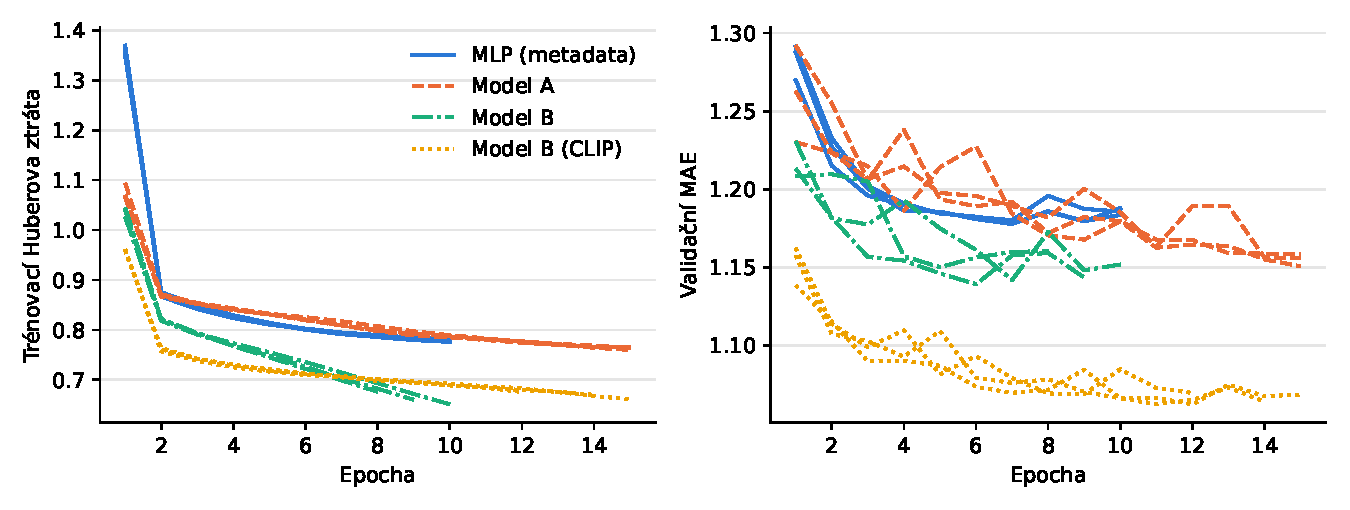
\includegraphics[width=\textwidth]{krivky.pdf}
    \caption{Trénovací Huberova ztráta (vlevo) a validační MAE (vpravo) po epochách,
    všechny tři seedy každého modelu.}
    \label{fig:krivky}
\end{figure}

U modelu B trénovací ztráta dál klesá, zatímco validační MAE se po 5. až 7. epoše přestane
zlepšovat (obrázek~\ref{fig:krivky}). Hlava se začíná přeučovat a trénování ukončí early stopping.
Validační MAE modelu A kolísá, ale klesá až do poslední epochy a nejnižší je v 15. epoše u všech
tří seedů. Model A tedy spíše nebyl dotrénován a limit počtu epoch ho mohl omezit. Model
s encoderem CLIP má nižší validační chybu než ostatní modely už od první epochy.

\begin{figure}[h]
    \centering
    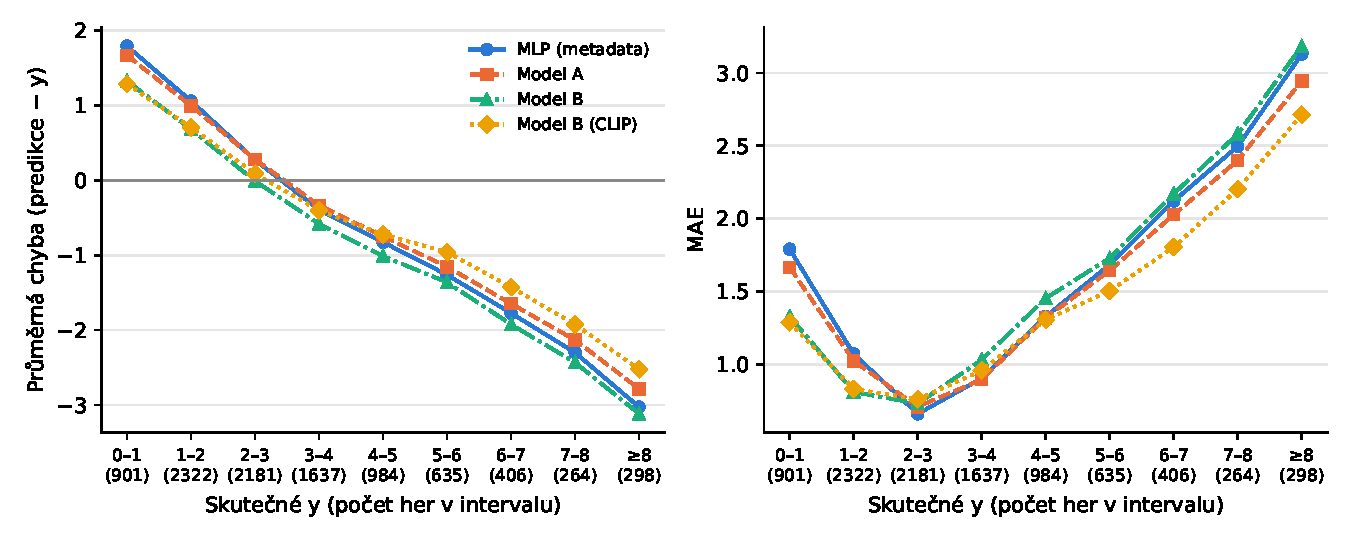
\includegraphics[width=\textwidth]{chyby.pdf}
    \caption{Průměrná chyba (predikce $-$ $y$, vlevo) a MAE (vpravo) na testovací množině podle
    skutečné hodnoty $y$. Chyba každé hry je zprůměrována přes tři seedy, v závorce je počet her
    v intervalu.}
    \label{fig:chyby}
\end{figure}

Všechny modely přeceňují hry s malým počtem recenzí a podceňují velmi populární hry
(obrázek~\ref{fig:chyby}), predikce jsou tedy stažené ke středu rozdělení. U her s $y \ge 8$ je průměrná chyba mezi $-2{,}5$ a $-3{,}1$,
skutečný počet recenzí je tedy přibližně 12- až 23krát vyšší než předpověď. Obrázky pomáhají
hlavně u málo populárních her: pro $y < 1$ je MAE nad samotnými metadaty 1,79, s modelem B 1,33
a s modelem s encoderem CLIP 1,29. Encoder CLIP jako jediný výrazněji zmenšuje podhodnocení
nejpopulárnějších her.

\subsection*{Výpočetní nároky}

\begin{table}[h]
    \centering
    \begin{tabular}{lrrrr}
        \toprule
        Model & Trénované parametry & Trénování [min] & Epocha [s] & Inference [her/s] \\
        \midrule
        MLP (metadata) & 10\,113 & 0,1 & 0,6 & 598\,152 \\
        Model A & 97\,809 & 58,4 & 233 & 1\,425 \\
        Model B & 54\,209 & 48,8 & 329 & 326 \\
        Model B (CLIP) & 37\,825 & 29,6 & 125 & 953 \\
        \bottomrule
    \end{tabular}
    \caption{Výpočetní nároky: průměr přes tři seedy, čas epochy jako medián.
    AMD Radeon RX 9070 XT (ROCm, Windows), bfloat16. Inference: dávka 128, 5 zahřívacích
    a 50 měřených průchodů, bez načítání dat.}
    \label{tab:naroky}
\end{table}

Model B má přibližně poloviční počet trénovaných parametrů než model A, každý průchod ale
počítá celý zmrazený ConvNeXt-Tiny (27,8 milionu parametrů), a jeho inference je proto přibližně
čtyřikrát pomalejší (tabulka~\ref{tab:naroky}). Celkový čas trénování modelu B je přesto kratší,
protože early stopping ho zastavil po 8 až 10 epochách. Model s encoderem CLIP
(87,9 milionu parametrů) trénoval i predikoval rychleji než model B. Čas epochy zahrnuje
načítání obrázků a validaci. Opakované měření inference se u modelu A lišilo o 27\,\%.

\section{Závěr}

Obrázky nesou o popularitě hry informaci, která v metadatech není. Oba hybridní modely mají
na validační i testovací množině nižší MAE než všechny baseline nad metadaty a ablace ukázala,
že kombinace obou modalit je lepší než každá zvlášť. Největší přínos měla volba předtrénovaného
encoderu: CLIP snížil testovací MAE modelu B z 1,183 na 1,108. Rozdíl mezi vlastní CNN
(model A) a zmrazeným ConvNeXt-Tiny (model B) je malý a při třech seedech jen orientační.

Encodery modelu B byly předtrénovány na velkém množství dalších dat s mnohem větším výpočetním
rozpočtem, nejde tedy o srovnání se stejným rozpočtem jako u modelu A. Hlavní omezení studie
jsou hledání hyperparametrů s jedním seedem a jen pro encoder ConvNeXt, limit 15 epoch, který
pravděpodobně omezil model A, a výstup modelů v bfloat16, který predikce zaokrouhluje
přibližně na 0,03. Všechny modely stahují predikce ke středu rozdělení a velmi populární hry
systematicky podhodnocují. Publikované výsledky nejsou přímo srovnatelné, protože se liší
čištění dat, definice cílové proměnné i rozdělení dat.
% TODO: ověřit, zda existují publikované výsledky na tomto datasetu

\subsection*{Využití generativní AI}

% TODO:


\printbibliography[title=Zdroje]

\end{document}